\section{GPS-tracks}

GPS-track is a common visual representation for machine path for some period of time. It can be used for detailed analysis of where and when the machine was located, what was the speed at concrete moment, where the stoppage has been occured etc.

This detailing analysis is useful when other more specific reports can not bring the necessary analysis granularity. For example, we need to determine the vehicle that travelled the most yesterday. In this case we use some aggregation report, possibly in tabular format, and sort the number of travelled kilometers descending. But why, where and exactly when the vehicle has been performed its route -- it can be analysed using GPS-tracks feature.

In figure~\ref{fig:11} the machine track for concrete period is shown. Whole track is divided on several regions which are commonly called ``clusters''. There are two types of clusters: 1) cluster with red marker which contain stoppages 2) cluster with blue ``directed'' marker with approximate direction of movement. The region is shown when the user hovers the cluster (figure~\ref{fig:11}). Cluster zooming can be done using single click action. 

\begin{figure}[H]
\centering
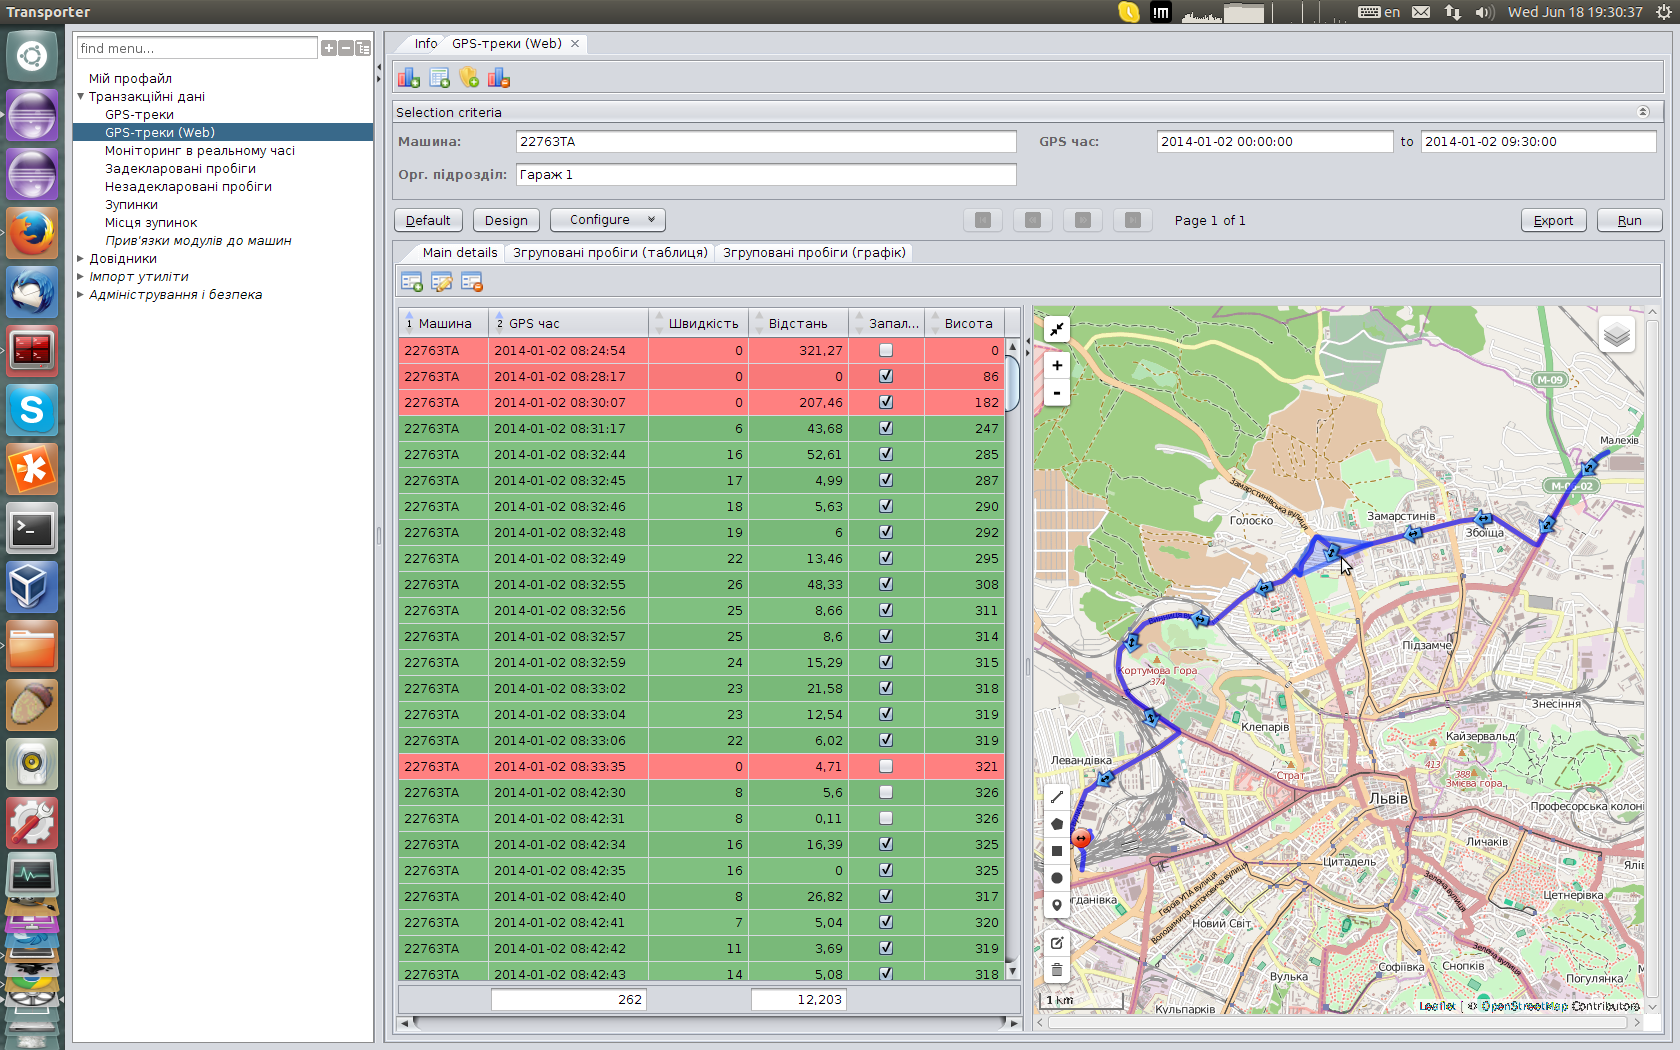
\includegraphics[width=\linewidth]{chapters/02-gpstracks/images/11-clusterised-gps-track-view-with-hovered-cluster.png}
\caption{Clusterised GPS-track view with hovered cluster}\label{fig:11}
\end{figure}

\newpage
Zooming to concrete region using clicking on a cluster is very handy and conveniently. Typical scenario of usage is to analyse which was the track in some particular place. The result of clicking is shown on figure~\ref{fig:12} -- the smaller part of track has been clusterised. The animation of nodes and map is used during zooming to better follow by zooming process.

\begin{figure}[H]
\centering
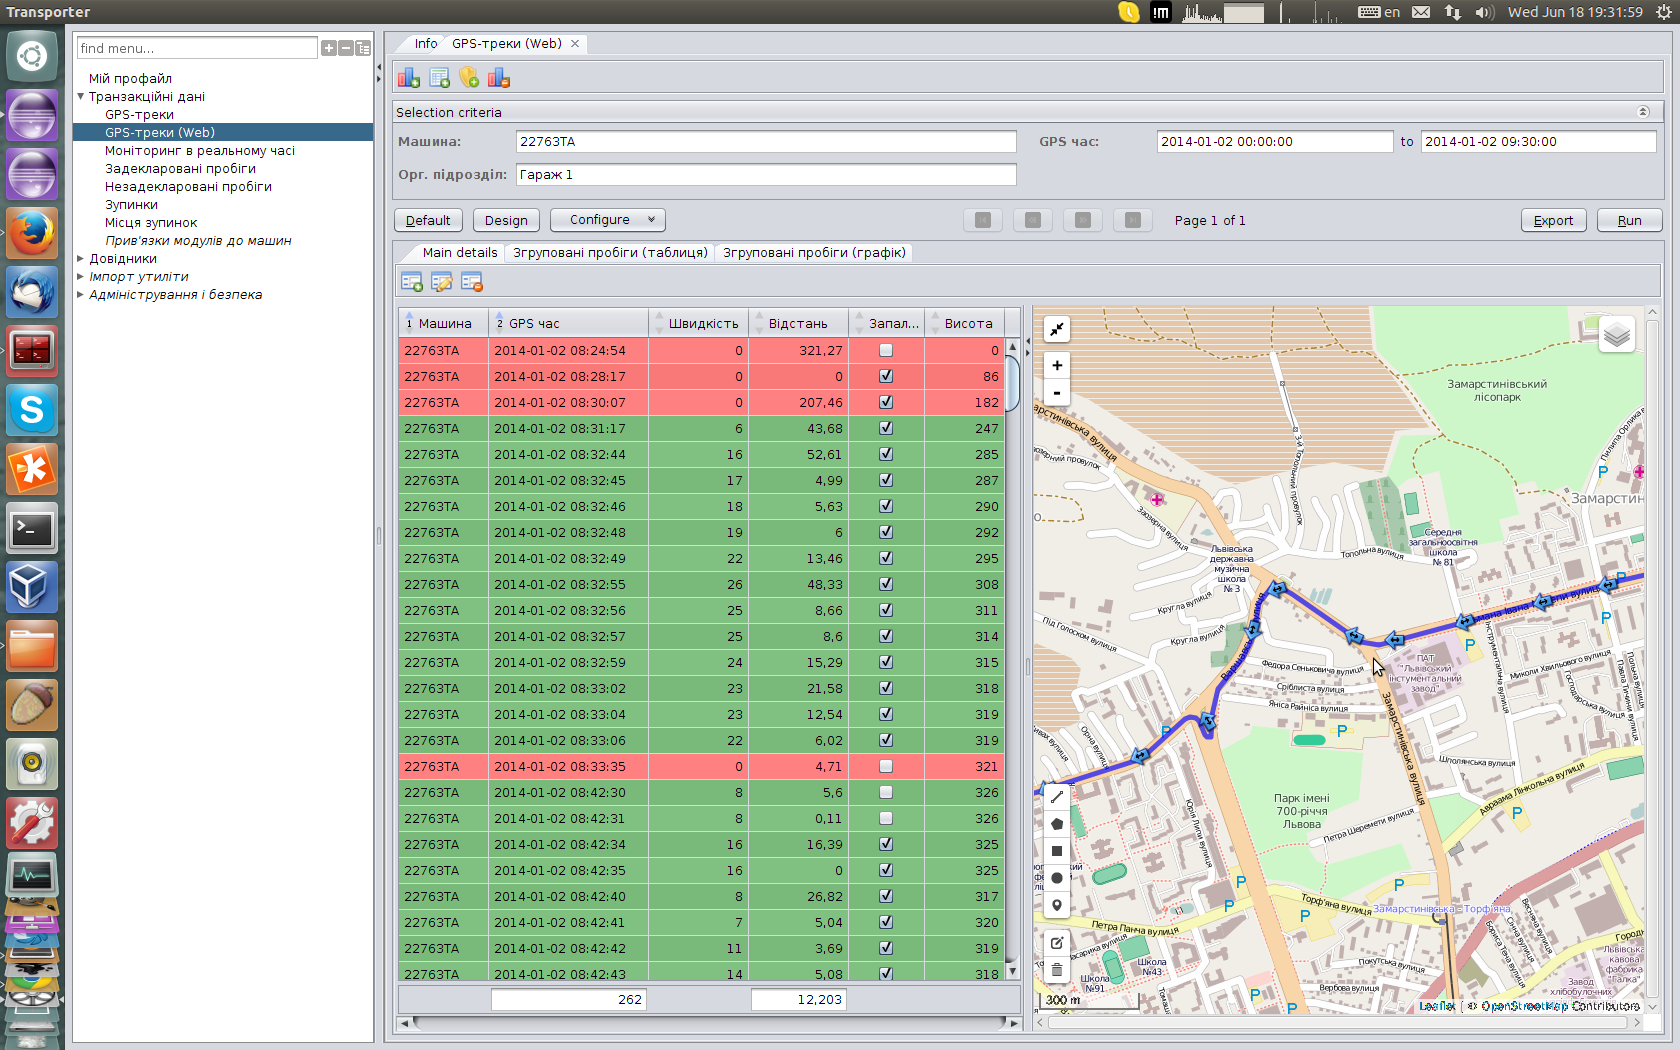
\includegraphics[width=\linewidth]{chapters/02-gpstracks/images/12-zooming-by-clicking-a-cluster.png}
\caption{Zoomed cluster region after the cluster has been clicked}\label{fig:12}
\end{figure}

\newpage
If the user clicks on some smaller cluster -- the detailed GPS-track is appeared with concrete GPS-messages (figure~\ref{fig:13}). The directions of the messages are precise enough to the level which GPS-module provides. 

\begin{figure}[H]
\centering
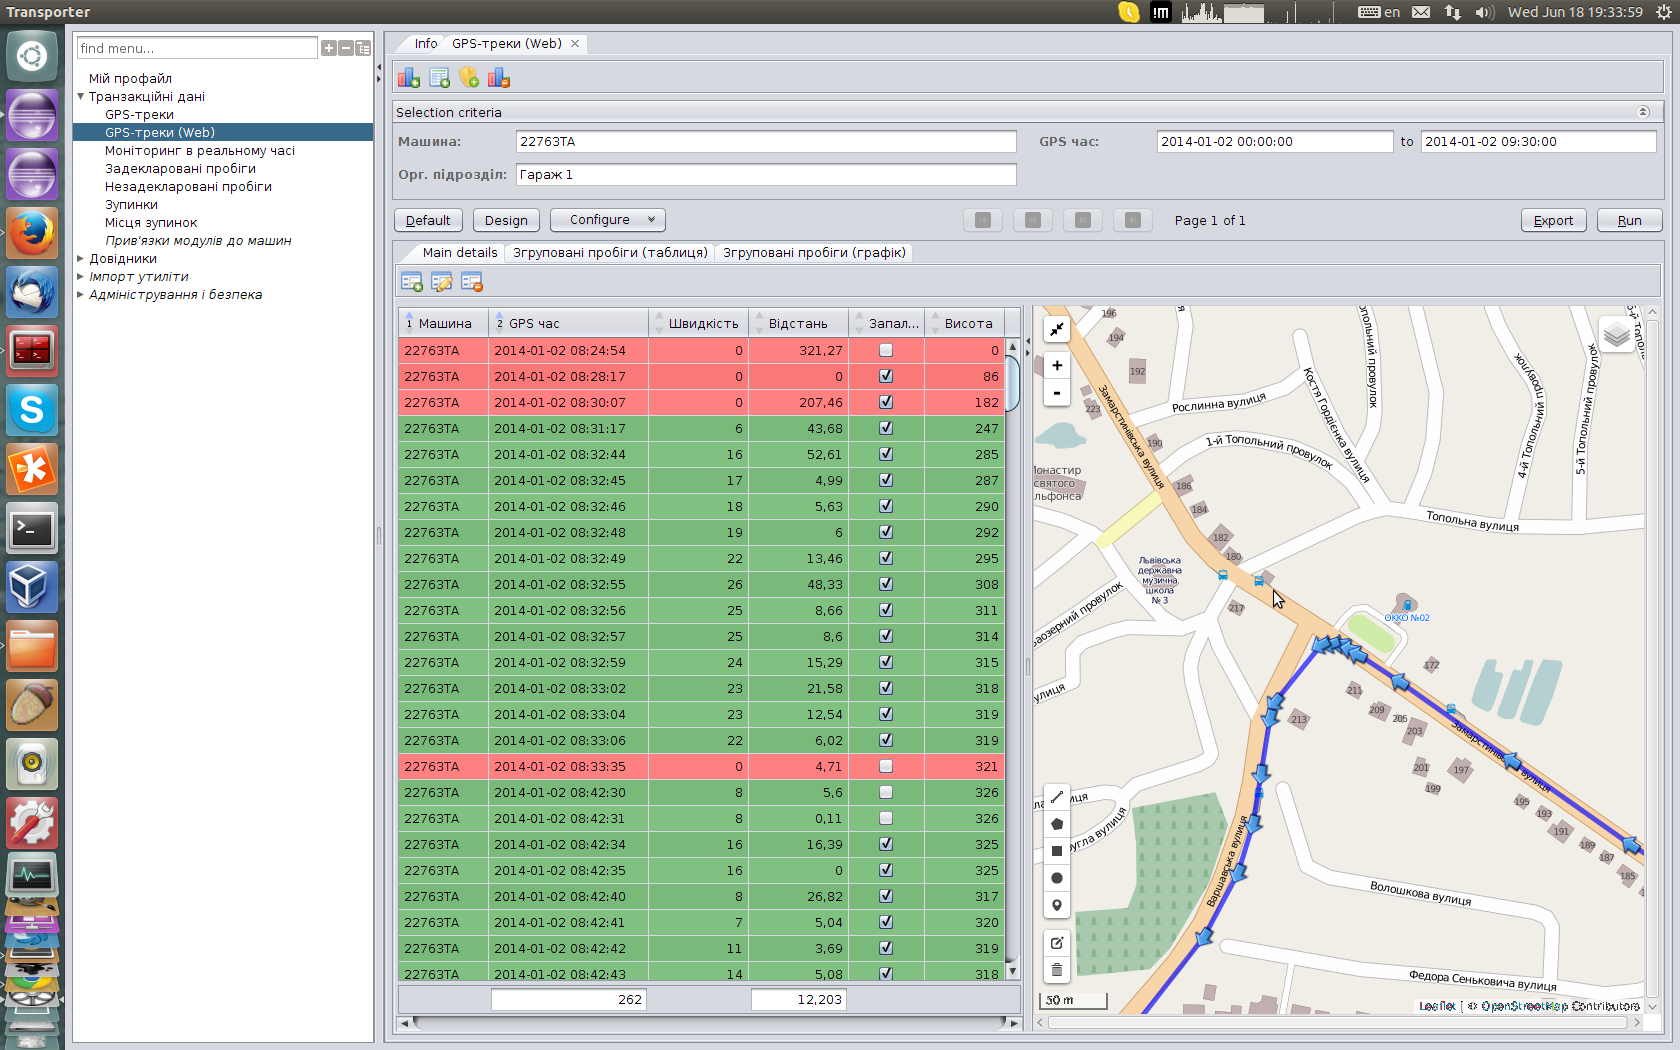
\includegraphics[width=\linewidth]{chapters/02-gpstracks/images/13-detailed-gps-track-view.png}
\caption{Detailed GPS-track view}\label{fig:13}
\end{figure}

\newpage
If the user clicks on red cluster -- the smaller part of track clusterises (figure~\ref{fig:14}). Small stoppage clusters are shown in this case which means that the vehicle made stoppages in all that places.

\begin{figure}[H]
\centering
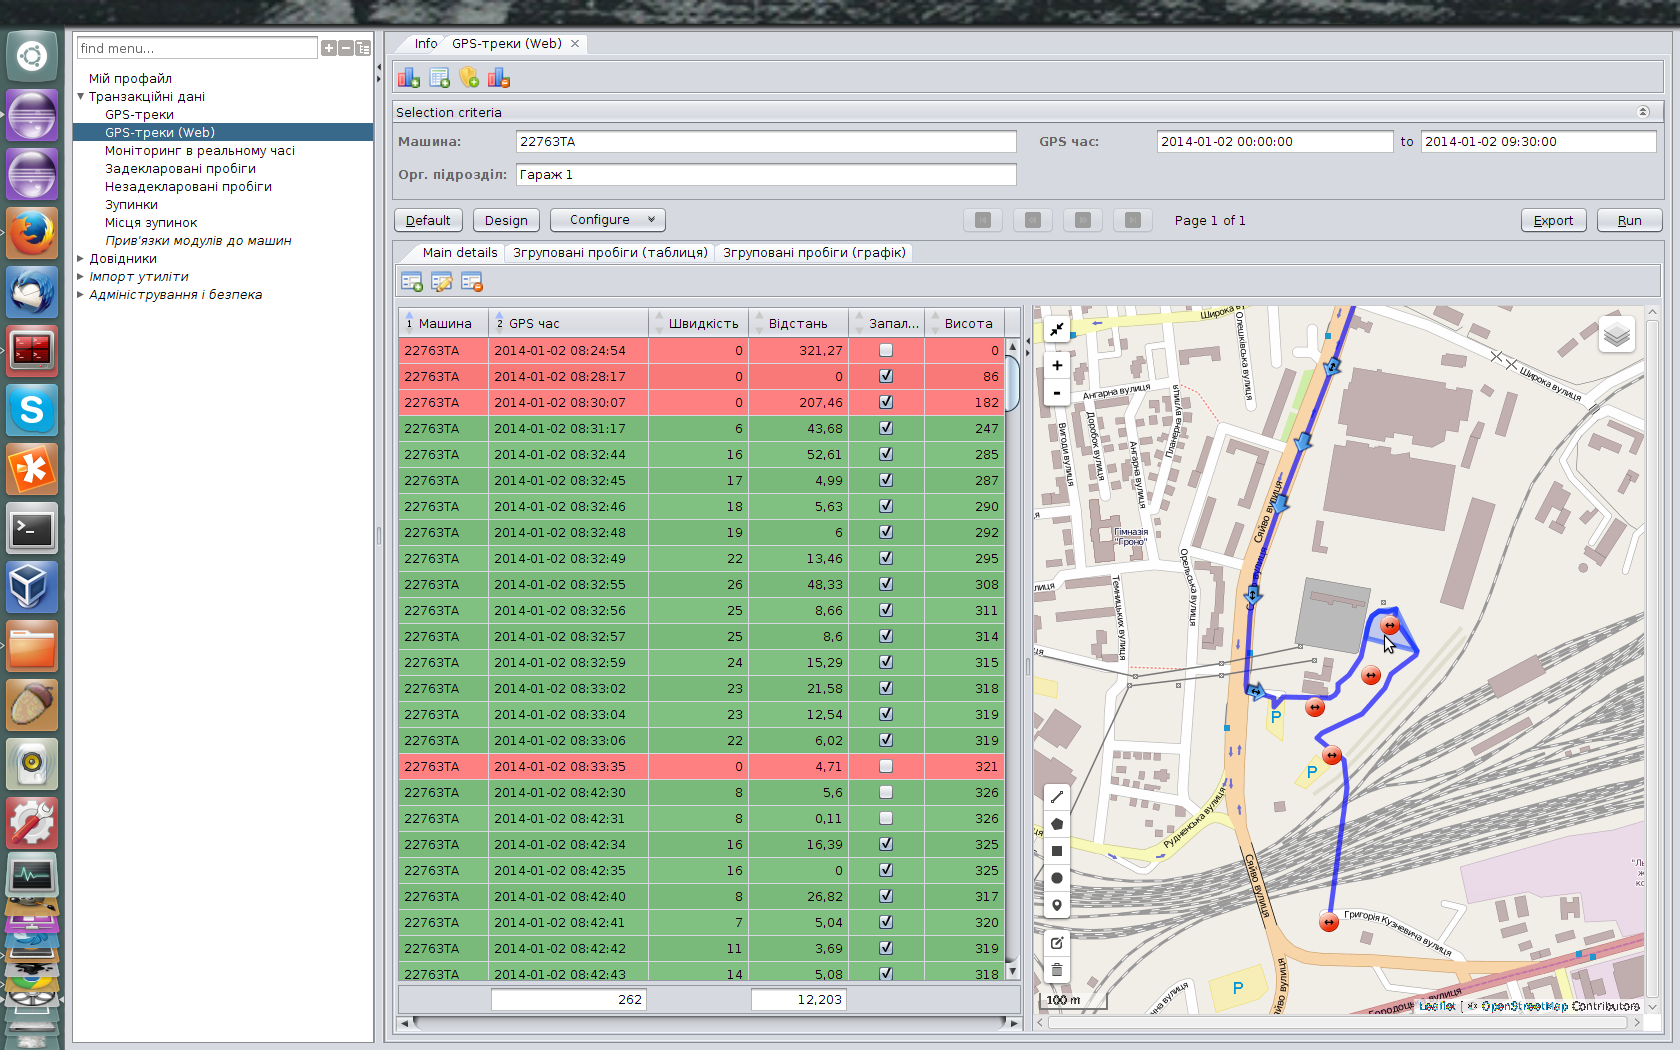
\includegraphics[width=\linewidth]{chapters/02-gpstracks/images/14-clusters-with-stoppage-messages-with-zero-speed.png}
\caption{Clusters with stoppage messages with zero speed}\label{fig:14}
\end{figure}

\newpage
If the user clicks on some smaller cluster -- the detailed GPS-track is appeared with concrete GPS-messages which include zero-speed messages (figure~\ref{fig:15}).

\begin{figure}[H]
\centering
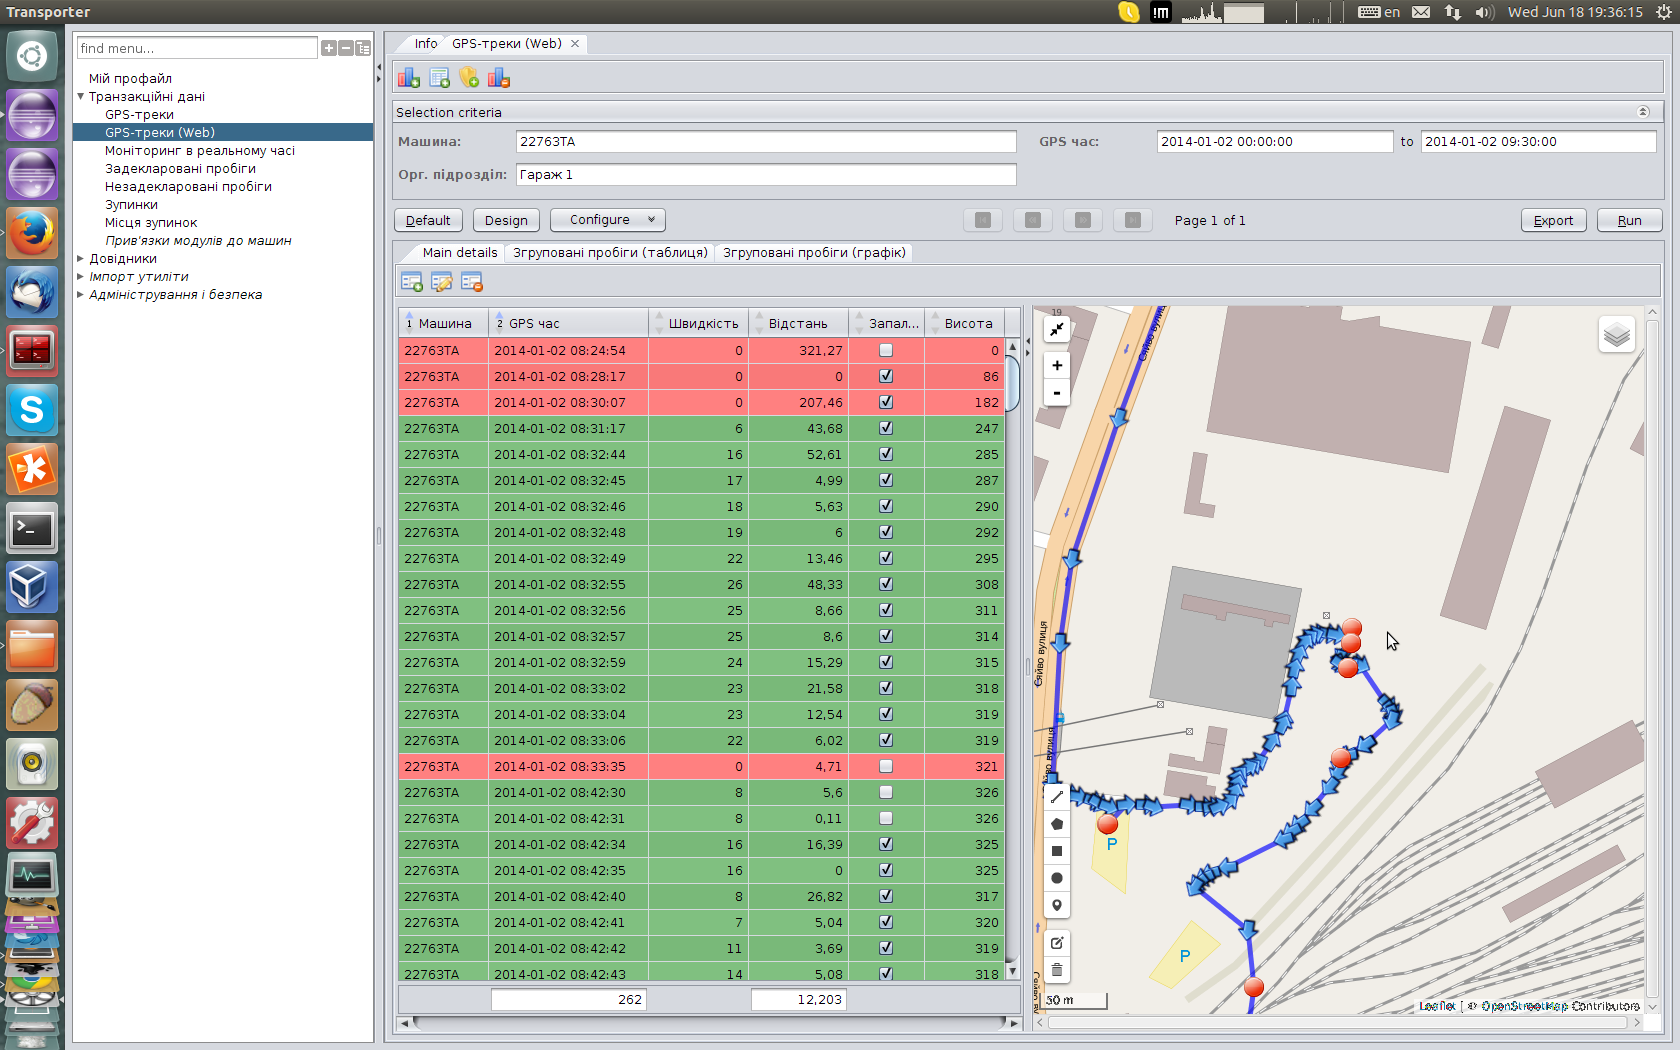
\includegraphics[width=\linewidth]{chapters/02-gpstracks/images/15-detailed-view-with-stoppages.png}
\caption{Detailed view with stoppages}\label{fig:15}
\end{figure}

\newpage
Concrete message details can be reviewed using message selection -- simple clicking action (figure~\ref{fig:16}). The popup shows and colouring of the message changes to green after selection. Please also note that appropriate grid row is also selected. 

If the user hovers the track messages they will appear to the top. Also the stoppage message is always on top to draw user's attention.

\begin{figure}[H]
\centering
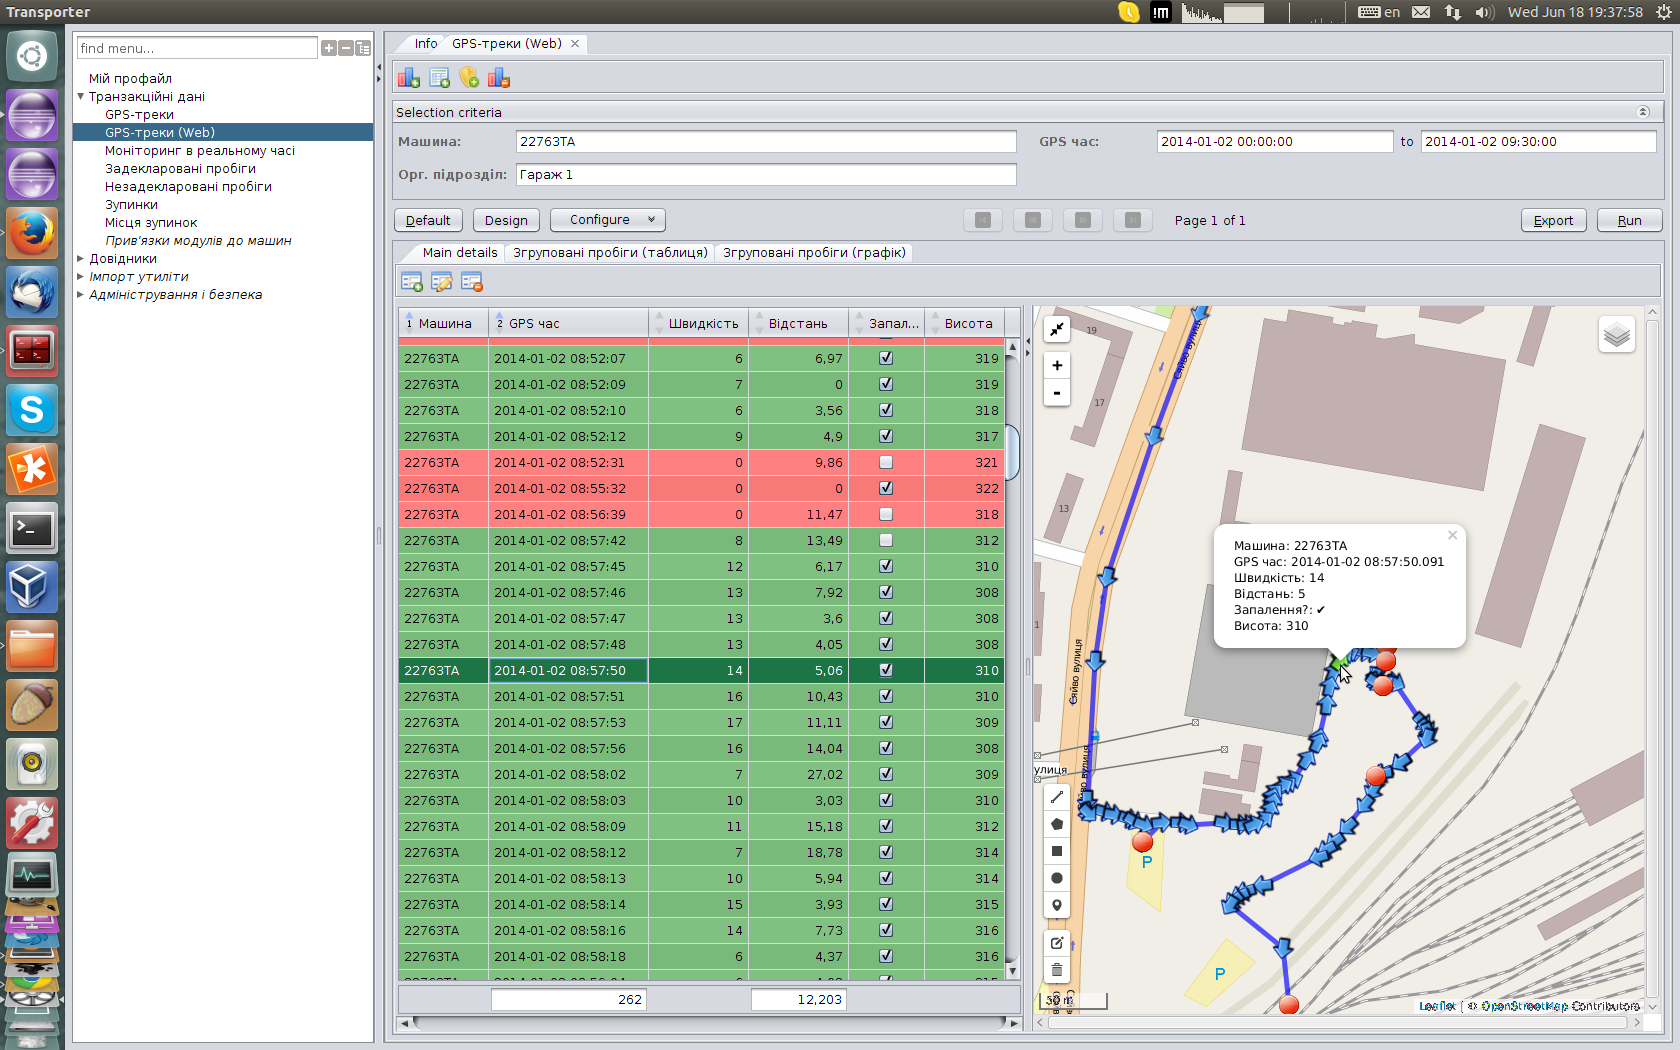
\includegraphics[width=\linewidth]{chapters/02-gpstracks/images/16-selected-message-with-popup.png}
\caption{Selected message with popup}\label{fig:16}
\end{figure}

\newpage
Selected stoppage message is shown on figure~\ref{fig:17}.

\begin{figure}[H]
\centering
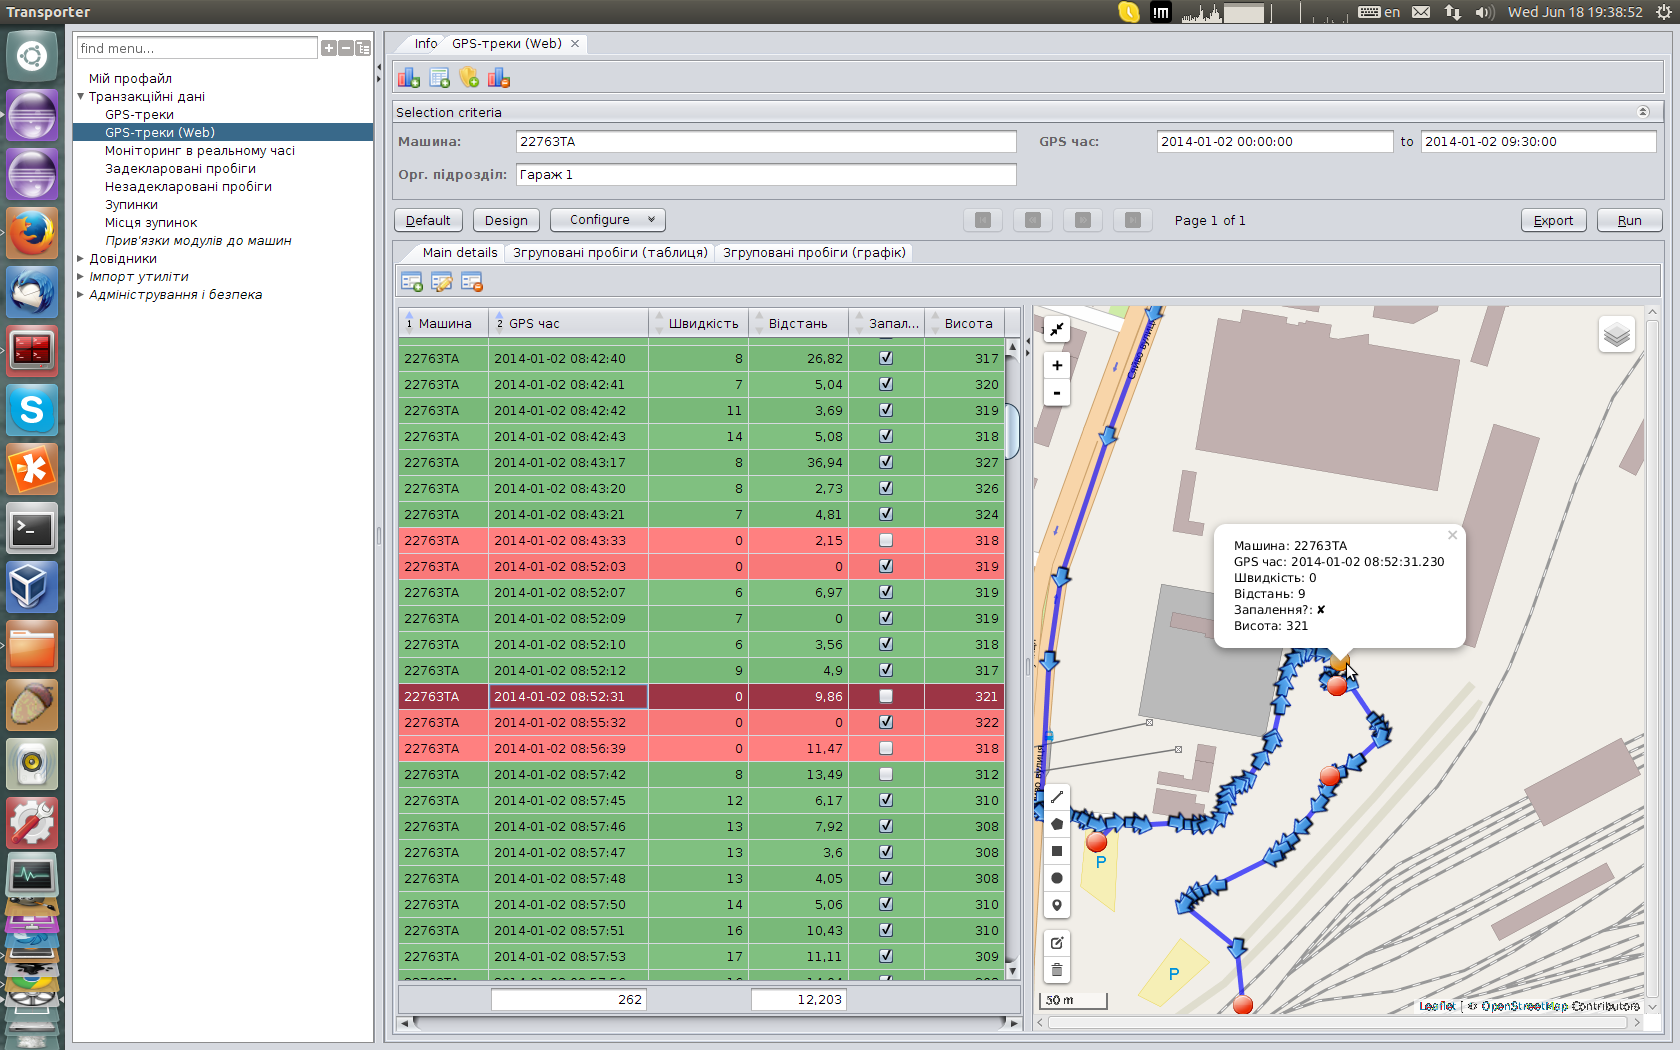
\includegraphics[width=\linewidth]{chapters/02-gpstracks/images/17-selected-stoppage-with-popup.png}
\caption{Selected stoppage message with popup}\label{fig:17}
\end{figure}

\newpage
The ability to show large GPS-tracks has been investigated and the results are shown on figure~\ref{fig:18}. Here the data from one machine for one month has been shown. It includes ~28000 messages and ~1500 kilometers of track movements. The performance is reasonable (at least for desktop browsers and TG java client, android browser client is somewhat slower).

\begin{figure}[H]
\centering
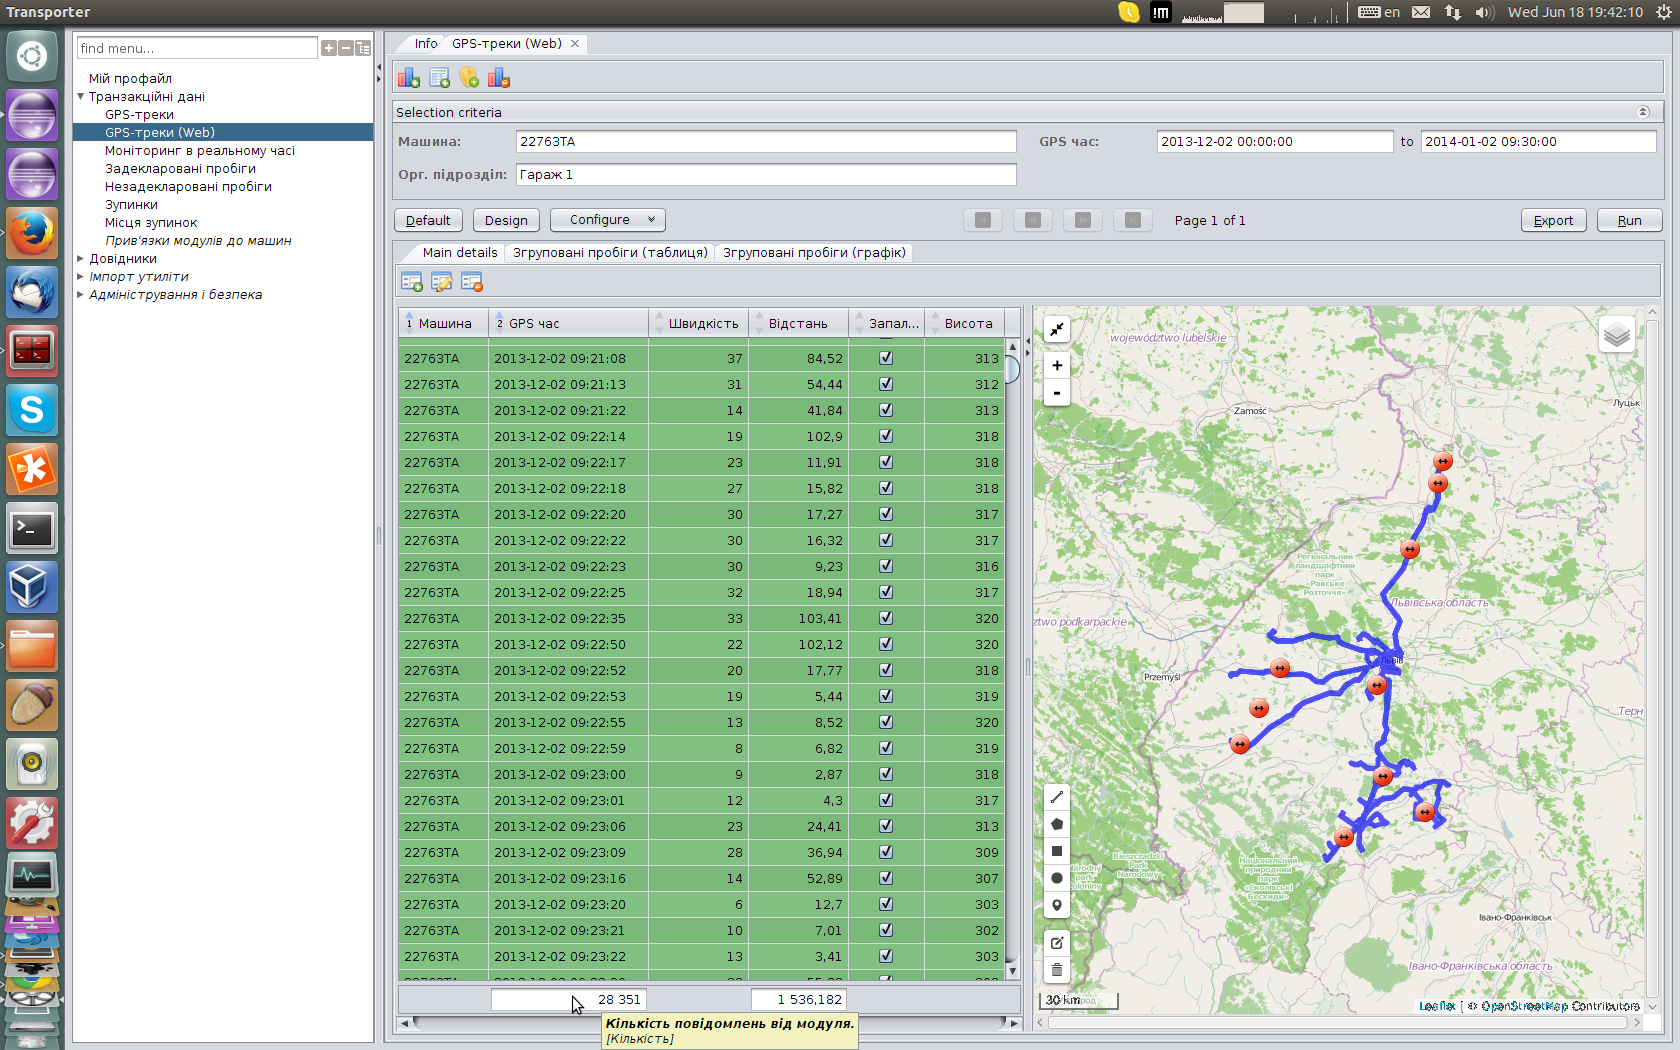
\includegraphics[width=\linewidth]{chapters/02-gpstracks/images/18-huge-dataset-processed-1machine-1month.png}
\caption{Large dataset processed (1 machine for 1 month)}\label{fig:18}
\end{figure}

\newpage
Large dataset details is shown on figure~\ref{fig:19} and figure ~\ref{fig:20}.

\begin{figure}[H]
\centering
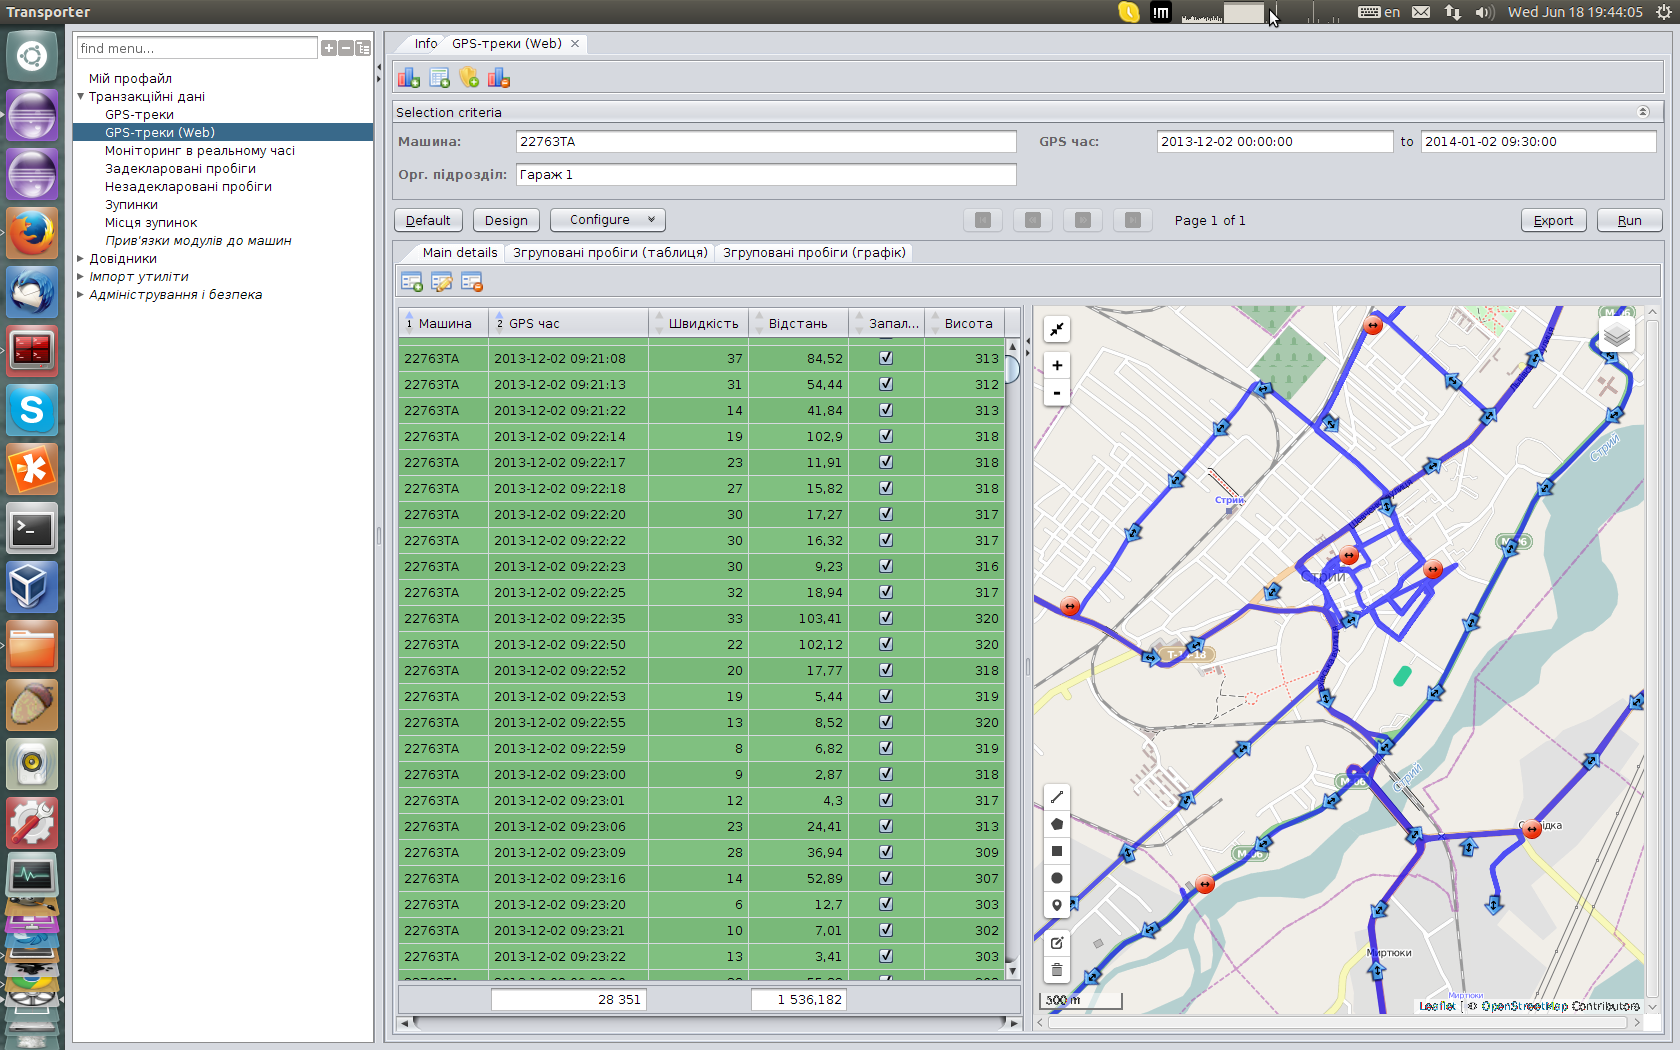
\includegraphics[width=\linewidth]{chapters/02-gpstracks/images/19-middle-details-at-some-place.png}
\caption{Middle details at some place}\label{fig:19}
\end{figure}

\begin{figure}[H]
\centering
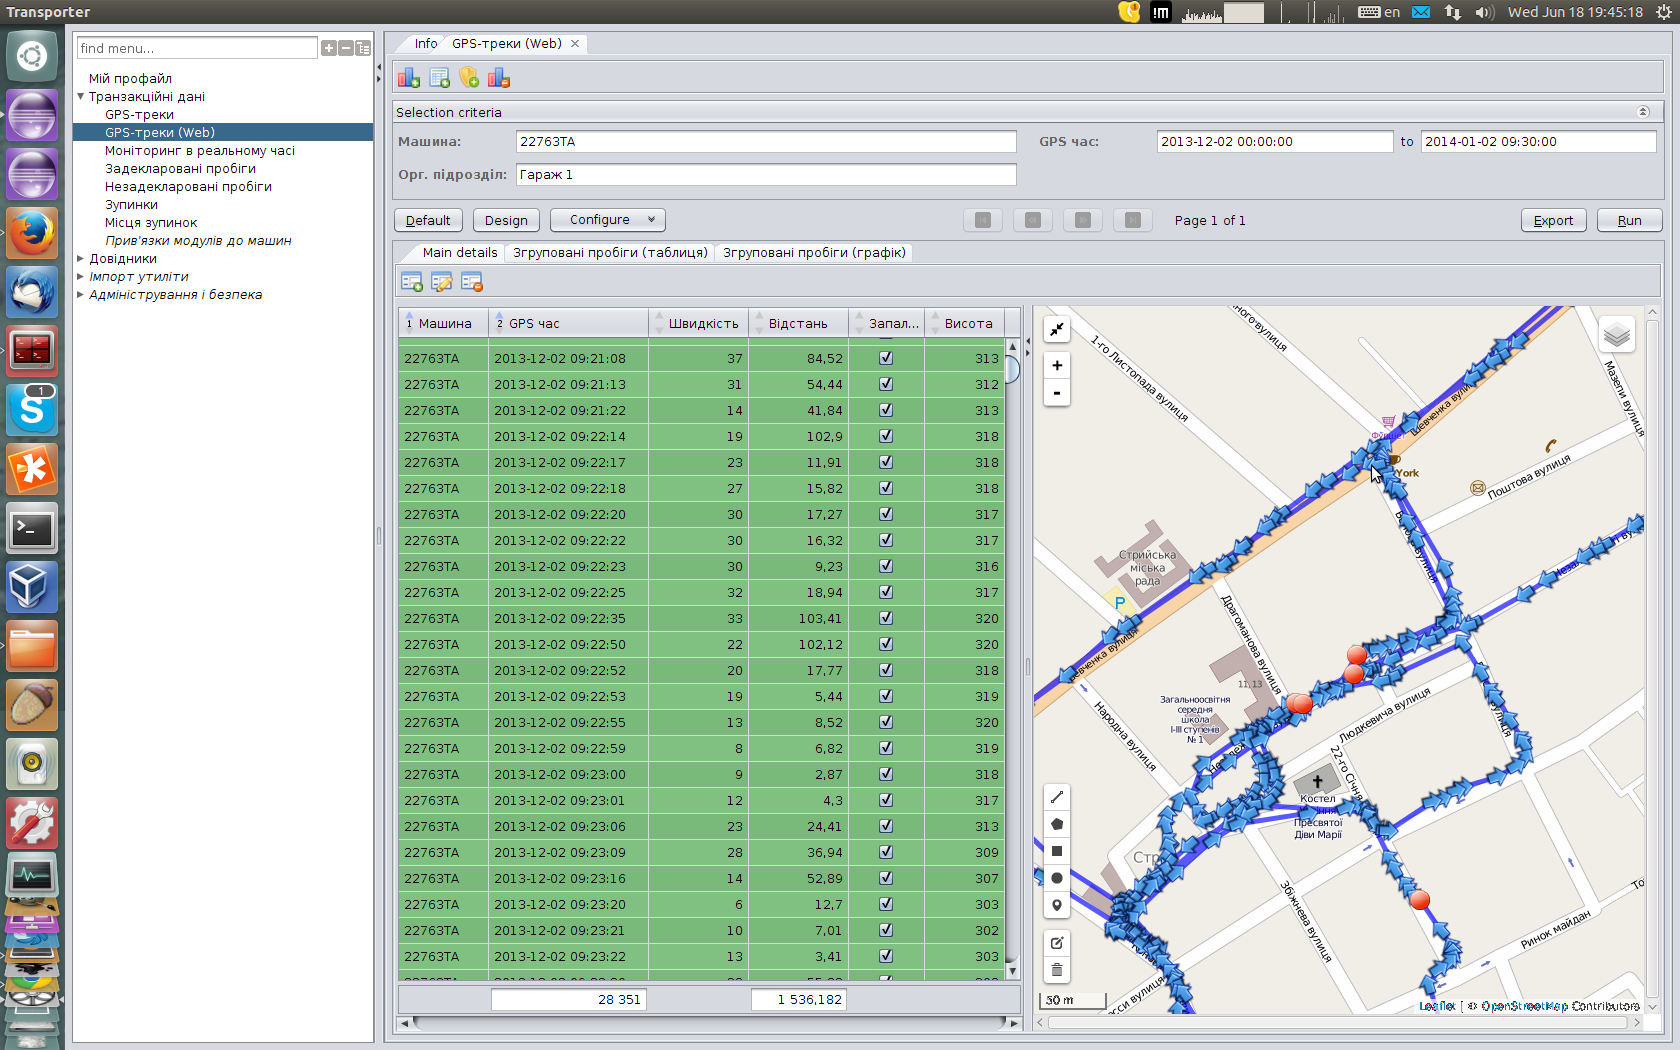
\includegraphics[width=\linewidth]{chapters/02-gpstracks/images/20-full-details-and-marker-hovering-feature.png}
\caption{Full details and marker hovering feature}\label{fig:20}
\end{figure}